\documentclass[letterpaper, 11pt]{article}
\usepackage{graphicx}
\usepackage{natbib}
\usepackage[left=3cm,top=3cm,right=3cm]{geometry}
\usepackage{parskip}
\usepackage{amsmath}

\renewcommand{\topfraction}{0.85}
\renewcommand{\textfraction}{0.1}

\newcommand{\hyperparams}{\boldsymbol{\alpha}}
\newcommand{\xx}{\mathbf{x}}

\title{Inference for Trans-dimensional Bayesian Models with Diffusive Nested
Sampling}
\author{Brendon J. Brewer}

\begin{document}
\maketitle
\abstract{This is the abstract.}

\section{Introduction}
\setlength{\parindent}{0cm}
\setlength{\parskip}{3mm}
Many inference problems have the following structure. There is some unknown
number, $N$, of objects in a region. Each of the $N$ objects has a property
$\xx$, which may be a single scalar value (for example, a mass), or a set of
values (e.g. a position and a mass).

We would like to assign a prior to the objects' properties $\{\xx_i\}_{i=1}^N$.
Since $N$ may be large, it is usually easier to assign an ``interim prior''
conditional on some hyperparameters $\hyperparams$, and then assign a prior to
$\hyperparams$. This kind of model is usually called {\it hierarchical}.

The prior for $N$, $\hyperparams$, and $\{\xx_i\}$ is usually factorised
in the following way:

\begin{eqnarray}
p(N, \hyperparams, \{\xx_i\}) &=& p(N) p(\hyperparams | N) p(\{\xx_i\} | \hyperparams, N) \\
&=& p(N) p(\hyperparams) \prod_{i=1}^N p(\xx_i | \hyperparams).
\end{eqnarray}

Here we have assumed the priors for $N$ and $\hyperparams$ are independent, and
the interim prior for $\{\xx_i\}$ is iid and does not depend on $N$.
Given data $\mathcal{D}$, we usually want to calculate properties of the
posterior distribution given by:
\begin{eqnarray}
p(N, \hyperparams, \{\xx_i\} | \mathcal{D}) \propto
p(N, \hyperparams, \{\xx_i\})
p(\mathcal{D} | N, \hyperparams, \{\xx_i\})\label{eq:bayes}
\end{eqnarray}
The general method used to calculate properties of the posterior distribution
is to generate samples from it using Markov Chain Monte Carlo (MCMC).

The marginal likelihood, or evidence, is also an important quantity, and is
the normalisation constant of the posterior given in Equation~\ref{eq:bayes}:
\begin{eqnarray}
\mathcal{Z} &=& p(\mathcal{D})\\
&=& \sum_{i=0}^{N_{\rm max}} \int
p(N, \hyperparams, \{\xx_i\})p(\mathcal{D} | N, \hyperparams, \{\xx_i\})
\, d^N \xx_i \, d\hyperparams \label{eq:evidence}
\end{eqnarray}


\begin{figure}
\begin{center}
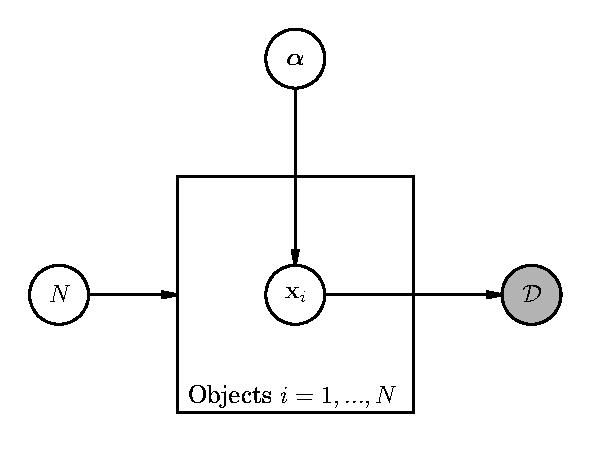
\includegraphics{pgm.pdf}
\caption{\it A probabilistic graphical model (PGM) depicting the kind
of model discussed in this paper. Produced using daft ({\tt daft-pgm.org}).
\label{fig:pgm}}
\end{center}
\end{figure}

In other studies, it has been common to do separate runs of Nested Sampling
$N$ fixed at various trial values. Then, the posterior for $N$ can be calculated
based on the estimates of the evidence obtained as a function of $N$. However,
in this paper, we use trans-dimensional MCMC moves to infer $N$. In other words,
$N$ is treated as just another parameter, and the marginal likelihood defined
in Equation~\ref{eq:evidence}, which we can compute, also includes the sum over
the unknown parameter $N$. Our motivation
for using Nested Sampling is not primarily to calculate $\mathcal{Z}$.
The motivation for using Nested Sampling, rather than just sampling the
posterior using trans-dimensional MCMC, is that the posterior often contains
difficult features, such as strong dependencies or multiple modes, that cause
problems with mixing. Diffusive Nested Sampling
(DNS) replaces the posterior distribution with an alternative target
distribution composed of a mixture of the prior distribution with other, more
constrained distributions. This is similar to the idea of simulated annealing,
where the target distribution is modified to something ``easier'', however,
the sequence of distributions used in Nested Sampling avoids some of the
problems with simulated annealing: in particular, there is no need to choose
a temperature schedule, and the method does not fail when phase transitions
are present.

%%%%%%%%%%%%%%%%%%%%%%%%%%%%%%%%%%%%%%%%%%%%%%%%%%%%%%%%%%%%%%%%%%%%%%%
% Consider having a section on what kind of ME constraint would lead  %
% to the same prior as a hierarchical model.                          %
%%%%%%%%%%%%%%%%%%%%%%%%%%%%%%%%%%%%%%%%%%%%%%%%%%%%%%%%%%%%%%%%%%%%%%%

% Consider terminology: "objects" vs. "components"

\section{Metropolis proposals for the general problem}
We will now define a set of proposal distributions that can be used to
sample the prior distribution
$p(N, \hyperparams, \{\xx_i\}) = p(N) p(\hyperparams) \prod_{i=1}^N p(\xx_i | \hyperparams)$.
These proposals will need to satisfy detailed balance in order to be valid
when used inside DNS. When the proposal satisfies detailed balance with respect
to the prior, the DNS algorithm can incorporate hard likelihood constraints by
rejecting any proposal whose likelihood does not satisfy the constraint.
The overall proposal is a mixture of all of the proposals listed here.

When using DNS,
the proposals typically should be very heavy tailed. When
DNS is exploring a distribution close to the prior, large proposals will
generally be needed to explore the prior efficiently.
When DNS is exploring a distribution constrained to
very high values of the likelihood function, much smaller proposals will be
appropriate. Rather than attempting expensive tuning (since the number of
distributions involved may number in the hundreds or even thousands), we will
apply the heavy tailed proposal distributions and simply accept that there will
be some waste. If a parameter $u$ has a uniform prior between 0 and 1, then
a heavy-tailed proposal is defined by:
\begin{eqnarray}
u' &=& \textnormal{mod}\left(u + 10^{1.5 - 6a}b, 1\right)
\end{eqnarray}
where $a \sim \textnormal{Uniform}(0, 1)$ and $b\sim \mathcal{N}(0,1)$.
This is like a standard gaussian/normal random walk proposal, but with a
non-fixed step size, resulting in a scale mixture of normals.
When
$a$ is close to zero, the size of the proposal is of order 10, which (because
of the mod function) effectively randomises $u'$ from the prior. If $a$ is
close to 1, the scale of the proposal is roughly $10^{-4}$ times the prior
width. The coefficient of $a$ was set to 6 because smaller proposals are
usually not necessary. The value 1.5 in the exponent was found to optimize the
performance of this proposal when sampling from $U(0, 1)$ and $\mathcal{N}(0,1)$
priors.

Most of the proposals involve changing one (or a subset) of the parameters
and/or hyperparameters while keeping the others fixed.

\subsection{Proposals that modify $N$}\label{sec:proposal1}
The first kind of proposal we consider are proposals that change the
dimension of the model, i.e. proposals that change the value of $N$. By
necessity, these will also change the parameters $\{\xx_i\}_{i=1}^N$ because
the number of parameters will be changed. The proposals used here are
traditionally called {\it birth and death} proposals.

We will assume that the prior for $N$ is a discrete uniform distribution
between 0 and some $N_{\rm max}$, inclusive. The proposal starts by choosing
a new value $N'$ according to
\begin{eqnarray}
N' &=& \textnormal{mod}\left(N + \delta_N, N_{\rm max} + 1\right)
\end{eqnarray}
where $\delta_N$ is drawn from a heavy tailed
distribution. The most probable values of $\delta_N$ are $\pm 1$, but values
of order $N_{\rm max}$ also have some probability, to allow fast exploration
when the target distribution is similar to the prior.

If $N' > N$, the extra parameters needed, $\{\xx_i\}_{i=N+1}^{N'}$,
are drawn from their prior conditional on the current value of the
hyperparameters, i.e. the interim prior $p(\xx | \hyperparams)$.

If $N' < N$, then $N - N'$ objects must be removed from the model. All
of the objects have the same probability of being selected for removal.

\subsection{Proposals that modify objects}\label{sec:proposal2}
We now consider a proposal distribution that modifies one or more of the
objects $\{\xx_i\}$, while keeping the number of objects $N$, as well as the
hyperparameters $\hyperparams$, fixed.

Let $F(x; \hyperparams)$ be a function that takes an object $x$ and transforms it
to a value $u$ that has a uniform distribution between 0 and 1, given $\hyperparams$.
If the object $x$ consists of a single scalar value, $F$ is the cumulative
distribution of the interim prior. Denote the inverse of $F$ by $G$.

A proposal
for an object involves transforming its parameters to $[0, 1]$ using $F$,
making the proposal in terms of $u$, and then transforming back.
Specifically, the proposal chooses
a new value $\xx_i'$ from the current value $\xx_i$ as follows:
\begin{eqnarray}
u_i &:=& F(\xx_i; \hyperparams)\\
u_i' &:=& \textnormal{mod}\left(u_i + \delta_u, 1\right)\\
\xx_i' &:=& G(u_i'; \hyperparams).
\end{eqnarray}
where $\delta_u$ is drawn from a heavy-tailed distribution.

Choosing just one object to change is most appropriate when the DNS
distribution is very constrained. When it is close to the prior, bolder
proposals that change more than one object at a time are possible. Hence,
we choose the number of objects to change from a heavy tailed distribution
wherer the most probable value is 1 but there is also a nontrivial probability
of proposing to change $\sim N$ objects at once.

\subsection{Proposals that change the hyperparameters,
keeping the objects fixed}\label{sec:proposal3}
Another kind of proposal that we will consider is a proposal that keeps all of
the objects fixed in place (i.e. leaves $\{\xx_i\}$) unchanged, but changes
the hyperparameter(s) from their current value $\hyperparams$
to a new value $\hyperparams'$. The proposal for the hyperparameter(s) is chosen
to satisfy detailed balance with respect to $p(\hyperparams)$.

The overall Metropolis acceptance probability
for this kind of move, if sampling the prior (or the constrained prior of DNS)
must include the following factor:
\begin{eqnarray}
\frac{\prod_{i=1}^N p(\xx_i | \hyperparams')}{\prod_{i=1}^N p(\xx_i | \hyperparams)}
\label{eqn:acceptance_prob}
\end{eqnarray}
Since this proposal leaves the objects $\{\xx_i\}$ fixed, it will usually not
affect the value of the likelihood, and therefore the likelihood will not need
to be recomputed.

\subsection{Proposals that change the hyperparameters
and all of the objects}\label{sec:proposal4}
The above proposals allow for changes to $N$, $\hyperparams$, and $\{\xx_i\}$,
and are therefore sufficient to allow for ``correct'' exploration of the
prior distribution, and the constrained prior distributions used in DNS.
However, they do not necessarily allow for {\it efficient} exploration, even
of the prior itself. The main reason for this is the inability for large
changes to be made to the hyperparameters $\hyperparams$. If the proposed change
from $\hyperparams$ to $\hyperparams'$ is large, the ratio in
Equation~\ref{eqn:acceptance_prob} is likely to be very small, and the move
will probably be rejected.

Therefore, we allow an additional move that changes $\hyperparams$ to a new
value $\hyperparams'$, but rather than leaving the objects $\{\xx_i\}$ fixed, we
drag them so they represent the distribution $p(\xx | \hyperparams')$ rather than
$p(\xx|\hyperparams)$. We do this by making use of the transformation functions
$F(x; \hyperparams)$ and $G(x; \hyperparams)$ defined in Section~\ref{sec:proposal2}.

The ``dragging'' process works as follows, and must be carried out on
each object:
\begin{eqnarray}
u_i &:=& F(\xx_i; \hyperparams)\\
\xx_i' &:=& G(\xx_i; \hyperparams')
\end{eqnarray}

\section{Sinusoidal example}
In this section we demonstrate a seemingly simple example which exhibits
a phase transition, making a standard MCMC approach difficult. Suppose
a signal is composed of $N$ sinusoids, of different periods, amplitudes,
and phases. The signal is observed at various times $\{t_i\}_{i=1}^N$ with
noise, and we want to use the resulting data to infer the number of sinusoids
$N$, along with the periods $\{T_i\}_{i=1}^N$, amplitudes $\{A_i\}_{i=1}^N$,
and phases $\{\phi_i\}_{i=1}^N$.
This kind of model has many applications, and has been solved analytically
under certain sets of assumptions \citep[see e.g.][]{bretthorst}.

The model for the signal is
\begin{eqnarray}
y(t) &=& \sum_{i=1}^N A_i \sin \left(\frac{2\pi t}{T_i} + \phi_i\right)
\end{eqnarray}
where there are $N$ sinusoids in the signal, the
amplitudes are $\{A_i\}$, the periods are $\{T_i\}$, and the phases are
$\{\phi_i\}$.

The sampling distribution (probability distribution for the data given the
parameters) is a normal (gaussian) distribution with mean zero and standard
deviation $\sigma$, applied independently to each data point:
\begin{eqnarray}
Y_i | N, \{A_i\}, \{T_i\}, \{\phi_i\} \sim
\mathcal{N}\left(\mu(t_i), \sigma^2\right).
\end{eqnarray}
We simulated some data based on the assumption $N=2$.
The simulated data is shown in Figure~\ref{fig:sinewave_data}, and shows a
large, low period oscillation with a smaller, much faster oscillation
superimposed. The noise level is such that the fast oscillation is difficult
to detect. The true values of the parameters were
$N=2$, $\mathbf{A} = \{1, 0.3\}$,
$\mathbf{T}=\{30, 2\}$, and $\boldsymbol{\phi} = \{0, 1\}$. The signal was
observed at $n=1001$ points equally spaced between $t=0$ and $t=100$.
The true form of the signal is:
\begin{eqnarray}
y(t) = \sin\left(\frac{2\pi t}{30}\right) +
0.3 \sin\left(\frac{2\pi t}{2} + 1\right)
\end{eqnarray}
and the noise standard deviation was $\sigma = 1$. The data $\{Y_i\}_{i=1}^n$
is displayed in Figure~\ref{fig:sinewave_data}.

\begin{figure}
\begin{center}
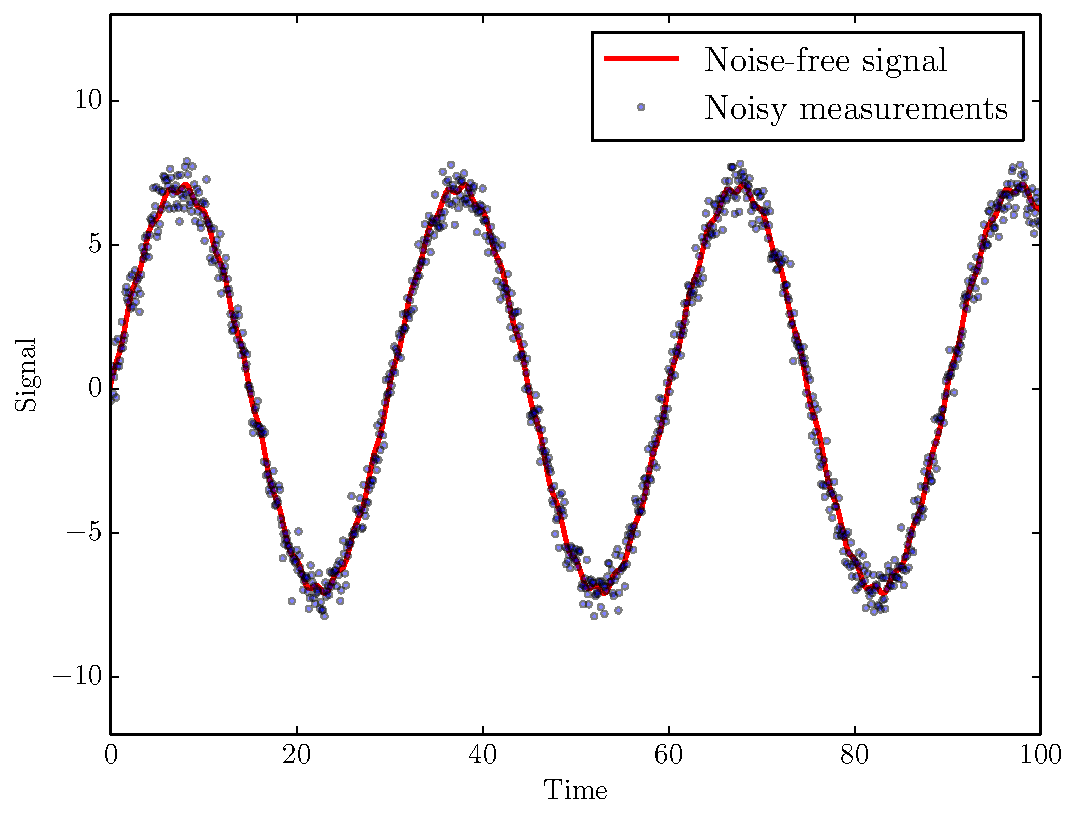
\includegraphics[scale=0.5]{sinewave_data.pdf}
\caption{The simulated data for the sinusoidal example. The solid line shows
the true signal and the points are the measurements, simulated based on a
noise standard deviation of $\sigma = 1$.
\label{fig:sinewave_data}}
\end{center}
\end{figure}

\begin{figure}
\begin{center}
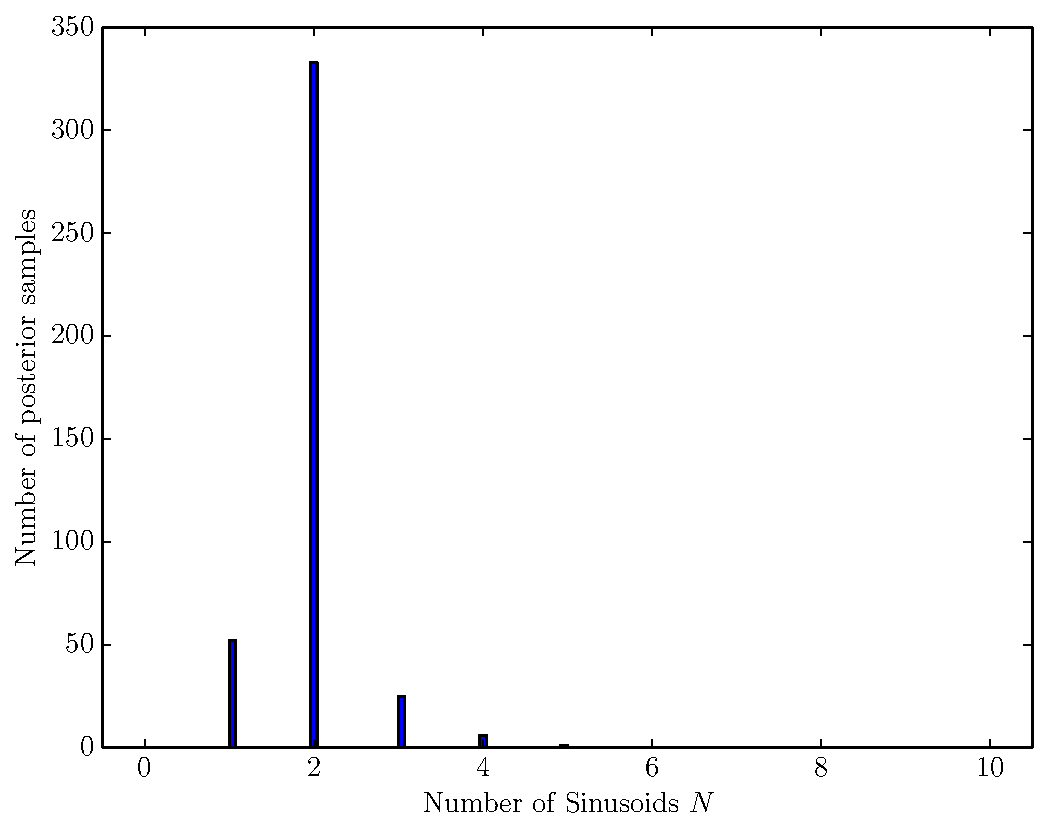
\includegraphics[scale=0.5]{N_result.pdf}
\caption{The inference for $N$, the number of sinusoids, based on the
sinusoid data. The true value was $N=2$.
\label{fig:N_result}}
\end{center}
\end{figure}

%\section{``Transit'' Example}
%\section{``Asteroseismology'' Example}
%\section{``Galaxy Field'' Example}




\section*{Acknowledgements}
This work is supported by a Marsden Fast-Start grant
from the Royal Society of New Zealand. I would like to thank the following
people for valuable conversations and inspiration:
Anna Pancoast (UCSB), David Hogg (NYU), Daniel Foreman-Mackey (NYU),
Courtney Donovan (Auckland), Tom Loredo (Cornell), Iain Murray (Edinburgh),
John Skilling (MaxEnt Data Consultants), and Daniela Huppenkothen
(Amsterdam, NYU).


\begin{thebibliography}{}

\bibitem[Bretthorst(1988)]{bretthorst} Bretthorst, G.~Larry.\  1988.\
Bayesian Spectrum Analysis and Parameter Estimation.\ In Lecture Notes in
Statistics, 48, Springer-Verlag, New York, New York.

\bibitem[Brewer et al.(2007)]{2007ApJ...654..551B} Brewer, B.~J., Bedding, 
T.~R., Kjeldsen, H., Stello, D.\ 2007.\ Bayesian Inference from 
Observations of Solar-like Oscillations.\ The Astrophysical Journal 654, 
551-557. 

\bibitem[Brewer et al.(2013)]{2013AJ....146....7B} Brewer, B.~J., 
Foreman-Mackey, D., Hogg, D.~W.\ 2013.\ Probabilistic Catalogs for Crowded 
Stellar Fields.\ The Astronomical Journal 146, 7. 

\bibitem[\protect\citeauthoryear{Brewer, P{\'a}rtay,
\& Cs{\'a}nyi}{2011b}]{dnest} Brewer B.~J., P{\'a}rtay L.~B., Cs{\'a}nyi G., 2011,
Statistics and Computing, 21, 4, 649-656. arXiv:0912.2380

\bibitem[Brewer et al.(2011)]{2011MNRAS.412.2521B} Brewer, B.~J., Lewis,
G.~F., Belokurov, V., Irwin, M.~J., Bridges, T.~J., Evans, N.~W.\ 2011.\
Modelling of the complex CASSOWARY/SLUGS gravitational lenses.\ Monthly
Notices of the Royal Astronomical Society 412, 2521-2529

\bibitem[\protect\citeauthoryear{Green}{1995}]{rjmcmc}
Green, P.~J., 1995, Reversible Jump Markov Chain Monte Carlo Computation and Bayesian Model Determination, Biometrika 82 (4): 711–732.

\bibitem[Neal(2001)]{neal} Neal, R.~M., 2001, 
Annealed importance sampling, Statistics and Computing, vol. 11, pp. 125-139.

\bibitem[\protect\citeauthoryear{Skilling}{1998}]{massinf}
Skilling J., 1998, Massive Inference and Maximum Entropy, in Maximum Entropy
and Bayesian Methods, Kluwer Academic Publishers, Dordrecht/Boston/London p.14

\bibitem[\protect\citeauthoryear{Skilling}{2006}]{skilling} Skilling, J., 2006, Nested Sampling for General Bayesian Computation, Bayesian Analysis 4, pp. 833-860.


\end{thebibliography}

\end{document}

